\documentclass[a4paper,11pt]{jsarticle}


% 数式
\usepackage{amsmath,amsfonts}
\usepackage{bm}
% 画像
\usepackage[dvipdfmx]{graphicx}
\usepackage{subcaption}


\begin{document}

\title{先端コンピューティング第3回レポート}
\author{03190895 材原貫太}
\date{\today}
\maketitle
\section*{課題1 canのFEMを実行する}
\begin{description}
  \item[境界条件]$\bullet$缶の下面に全方向の拘束
  \item[    ]$\bullet$xy平面に平行な缶の断面にz方向の拘束
  \item[    ]$\bullet$缶の内側に内圧を与える 
  \item[実行結果]
\end{description}
\begin{figure}[h] %hは hereの略
  \centering
  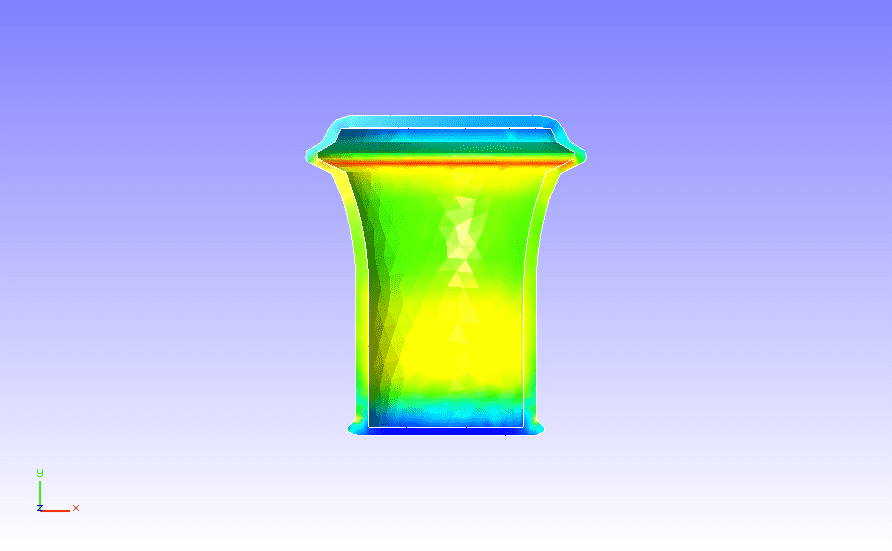
\includegraphics[height=5cm]{cancs_fistr_mises.png}
  \caption{ミーゼス応力のコンター図}
\end{figure}
\vspace{5cm}
\section*{課題2 capのFEMを実行する}
\begin{figure}[h]
  \begin{minipage}[b]{0.32\linewidth}
    \centering
    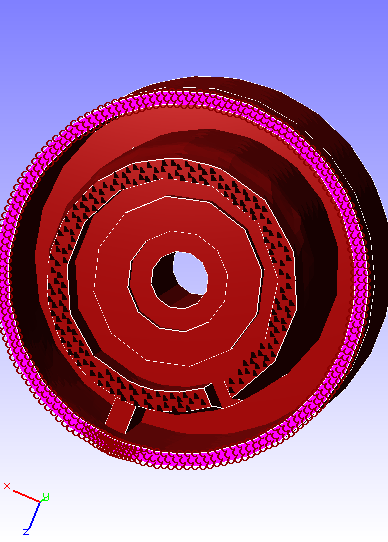
\includegraphics[scale=0.3]{cap_face03_boundary.png}
    \subcaption{全方向の拘束を与える}
  \end{minipage}
  \begin{minipage}[b]{0.32\linewidth}
    \centering
    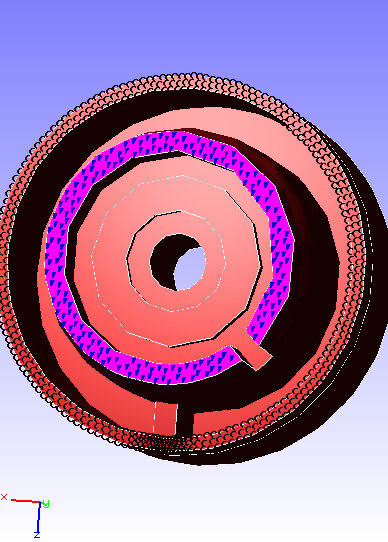
\includegraphics[scale=0.3]{cap_face010_dload.png}
    \subcaption{-1MPaの内圧を加える}
  \end{minipage}
  \begin{minipage}[b]{0.32\linewidth}
    \centering
    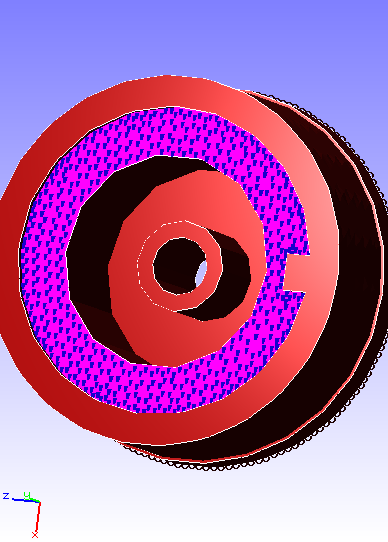
\includegraphics[scale=0.3]{cap_face08_dload.png}
    \subcaption{1MPaの内圧を加える}
  \end{minipage}
  \caption{境界条件}
\end{figure}
\begin{figure}[h]
  \centering
  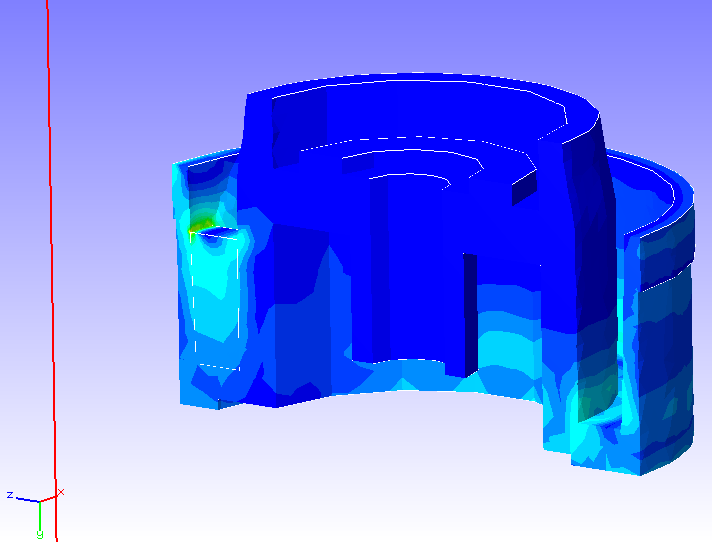
\includegraphics[scale=0.3]{cap_yz_mises.png}
  \caption{yz平面で切ったミーゼス応力のコンター図}
\end{figure}
\end{document}
